% Options for packages loaded elsewhere
\PassOptionsToPackage{unicode}{hyperref}
\PassOptionsToPackage{hyphens}{url}
\PassOptionsToPackage{dvipsnames,svgnames*,x11names*}{xcolor}
%
\documentclass[
  8pt,
  ignorenonframetext,
  dvipsnames]{beamer}
\usepackage{pgfpages}
\setbeamertemplate{caption}[numbered]
\setbeamertemplate{caption label separator}{: }
\setbeamercolor{caption name}{fg=normal text.fg}
\beamertemplatenavigationsymbolsempty
% Prevent slide breaks in the middle of a paragraph
\widowpenalties 1 10000
\raggedbottom
\setbeamertemplate{part page}{
  \centering
  \begin{beamercolorbox}[sep=16pt,center]{part title}
    \usebeamerfont{part title}\insertpart\par
  \end{beamercolorbox}
}
\setbeamertemplate{section page}{
  \centering
  \begin{beamercolorbox}[sep=12pt,center]{part title}
    \usebeamerfont{section title}\insertsection\par
  \end{beamercolorbox}
}
\setbeamertemplate{subsection page}{
  \centering
  \begin{beamercolorbox}[sep=8pt,center]{part title}
    \usebeamerfont{subsection title}\insertsubsection\par
  \end{beamercolorbox}
}
\AtBeginPart{
  \frame{\partpage}
}
\AtBeginSection{
  \ifbibliography
  \else
    \frame{\sectionpage}
  \fi
}
\AtBeginSubsection{
  \frame{\subsectionpage}
}
\usepackage{lmodern}
\usepackage{amssymb,amsmath}
\usepackage{ifxetex,ifluatex}
\ifnum 0\ifxetex 1\fi\ifluatex 1\fi=0 % if pdftex
  \usepackage[T1]{fontenc}
  \usepackage[utf8]{inputenc}
  \usepackage{textcomp} % provide euro and other symbols
\else % if luatex or xetex
  \usepackage{unicode-math}
  \defaultfontfeatures{Scale=MatchLowercase}
  \defaultfontfeatures[\rmfamily]{Ligatures=TeX,Scale=1}
\fi
% Use upquote if available, for straight quotes in verbatim environments
\IfFileExists{upquote.sty}{\usepackage{upquote}}{}
\IfFileExists{microtype.sty}{% use microtype if available
  \usepackage[]{microtype}
  \UseMicrotypeSet[protrusion]{basicmath} % disable protrusion for tt fonts
}{}
\makeatletter
\@ifundefined{KOMAClassName}{% if non-KOMA class
  \IfFileExists{parskip.sty}{%
    \usepackage{parskip}
  }{% else
    \setlength{\parindent}{0pt}
    \setlength{\parskip}{6pt plus 2pt minus 1pt}}
}{% if KOMA class
  \KOMAoptions{parskip=half}}
\makeatother
\usepackage{xcolor}
\IfFileExists{xurl.sty}{\usepackage{xurl}}{} % add URL line breaks if available
\IfFileExists{bookmark.sty}{\usepackage{bookmark}}{\usepackage{hyperref}}
\hypersetup{
  pdftitle={Data Analysis for Policy Research Using R},
  pdfauthor={Harold Stolper},
  colorlinks=true,
  linkcolor=Maroon,
  filecolor=Maroon,
  citecolor=Blue,
  urlcolor=blue,
  pdfcreator={LaTeX via pandoc}}
\urlstyle{same} % disable monospaced font for URLs
\newif\ifbibliography
\usepackage{color}
\usepackage{fancyvrb}
\newcommand{\VerbBar}{|}
\newcommand{\VERB}{\Verb[commandchars=\\\{\}]}
\DefineVerbatimEnvironment{Highlighting}{Verbatim}{commandchars=\\\{\}}
% Add ',fontsize=\small' for more characters per line
\usepackage{framed}
\definecolor{shadecolor}{RGB}{248,248,248}
\newenvironment{Shaded}{\begin{snugshade}}{\end{snugshade}}
\newcommand{\AlertTok}[1]{\textcolor[rgb]{0.94,0.16,0.16}{#1}}
\newcommand{\AnnotationTok}[1]{\textcolor[rgb]{0.56,0.35,0.01}{\textbf{\textit{#1}}}}
\newcommand{\AttributeTok}[1]{\textcolor[rgb]{0.77,0.63,0.00}{#1}}
\newcommand{\BaseNTok}[1]{\textcolor[rgb]{0.00,0.00,0.81}{#1}}
\newcommand{\BuiltInTok}[1]{#1}
\newcommand{\CharTok}[1]{\textcolor[rgb]{0.31,0.60,0.02}{#1}}
\newcommand{\CommentTok}[1]{\textcolor[rgb]{0.56,0.35,0.01}{\textit{#1}}}
\newcommand{\CommentVarTok}[1]{\textcolor[rgb]{0.56,0.35,0.01}{\textbf{\textit{#1}}}}
\newcommand{\ConstantTok}[1]{\textcolor[rgb]{0.00,0.00,0.00}{#1}}
\newcommand{\ControlFlowTok}[1]{\textcolor[rgb]{0.13,0.29,0.53}{\textbf{#1}}}
\newcommand{\DataTypeTok}[1]{\textcolor[rgb]{0.13,0.29,0.53}{#1}}
\newcommand{\DecValTok}[1]{\textcolor[rgb]{0.00,0.00,0.81}{#1}}
\newcommand{\DocumentationTok}[1]{\textcolor[rgb]{0.56,0.35,0.01}{\textbf{\textit{#1}}}}
\newcommand{\ErrorTok}[1]{\textcolor[rgb]{0.64,0.00,0.00}{\textbf{#1}}}
\newcommand{\ExtensionTok}[1]{#1}
\newcommand{\FloatTok}[1]{\textcolor[rgb]{0.00,0.00,0.81}{#1}}
\newcommand{\FunctionTok}[1]{\textcolor[rgb]{0.00,0.00,0.00}{#1}}
\newcommand{\ImportTok}[1]{#1}
\newcommand{\InformationTok}[1]{\textcolor[rgb]{0.56,0.35,0.01}{\textbf{\textit{#1}}}}
\newcommand{\KeywordTok}[1]{\textcolor[rgb]{0.13,0.29,0.53}{\textbf{#1}}}
\newcommand{\NormalTok}[1]{#1}
\newcommand{\OperatorTok}[1]{\textcolor[rgb]{0.81,0.36,0.00}{\textbf{#1}}}
\newcommand{\OtherTok}[1]{\textcolor[rgb]{0.56,0.35,0.01}{#1}}
\newcommand{\PreprocessorTok}[1]{\textcolor[rgb]{0.56,0.35,0.01}{\textit{#1}}}
\newcommand{\RegionMarkerTok}[1]{#1}
\newcommand{\SpecialCharTok}[1]{\textcolor[rgb]{0.00,0.00,0.00}{#1}}
\newcommand{\SpecialStringTok}[1]{\textcolor[rgb]{0.31,0.60,0.02}{#1}}
\newcommand{\StringTok}[1]{\textcolor[rgb]{0.31,0.60,0.02}{#1}}
\newcommand{\VariableTok}[1]{\textcolor[rgb]{0.00,0.00,0.00}{#1}}
\newcommand{\VerbatimStringTok}[1]{\textcolor[rgb]{0.31,0.60,0.02}{#1}}
\newcommand{\WarningTok}[1]{\textcolor[rgb]{0.56,0.35,0.01}{\textbf{\textit{#1}}}}
\usepackage{longtable,booktabs}
\usepackage{caption}
% Make caption package work with longtable
\makeatletter
\def\fnum@table{\tablename~\thetable}
\makeatother
\usepackage{graphicx,grffile}
\makeatletter
\def\maxwidth{\ifdim\Gin@nat@width>\linewidth\linewidth\else\Gin@nat@width\fi}
\def\maxheight{\ifdim\Gin@nat@height>\textheight\textheight\else\Gin@nat@height\fi}
\makeatother
% Scale images if necessary, so that they will not overflow the page
% margins by default, and it is still possible to overwrite the defaults
% using explicit options in \includegraphics[width, height, ...]{}
\setkeys{Gin}{width=\maxwidth,height=\maxheight,keepaspectratio}
% Set default figure placement to htbp
\makeatletter
\def\fps@figure{htbp}
\makeatother
\setlength{\emergencystretch}{3em} % prevent overfull lines
\providecommand{\tightlist}{%
  \setlength{\itemsep}{0pt}\setlength{\parskip}{0pt}}
\setcounter{secnumdepth}{-\maxdimen} % remove section numbering

%packages
\usepackage{graphicx}
\usepackage{rotating}
\usepackage{hyperref}

\usepackage{tikz} % used for text highlighting, amongst others
\usepackage{comment}

%title slide stuff
%\institute{Department of Education}
%\title{Managing and Manipulating Data Using R}

%
\setbeamertemplate{navigation symbols}{} % get rid of navigation icons:
\setbeamertemplate{footline}[page number]

%\setbeamertemplate{frametitle}{\thesection \hspace{0.2cm} \insertframetitle}
\setbeamertemplate{section in toc}[sections numbered]
%\setbeamertemplate{subsection in toc}[subsections numbered]
\setbeamertemplate{subsection in toc}{%
  \leavevmode\leftskip=3.2em\color{gray}\rlap{\hskip-2em\inserttocsectionnumber.\inserttocsubsectionnumber}\inserttocsubsection\par
}

%define colors
%\definecolor{uva_orange}{RGB}{216,141,42} % UVa orange (Rotunda orange)
\definecolor{mygray}{rgb}{0.95, 0.95, 0.95} % for highlighted text
	% grey is equal parts red, green, blue. higher values >> lighter grey
	%\definecolor{lightgraybo}{rgb}{0.83, 0.83, 0.83}

% new commands

%highlight text with very light grey
\newcommand*{\hlg}[1]{%
	\tikz[baseline=(X.base)] \node[rectangle, fill=mygray] (X) {#1};%
}
%, inner sep=0.3mm
%highlight text with very light grey and use font associated with code
\newcommand*{\hlgc}[1]{\texttt{\hlg{#1}}}

%modifying back ticks to add grey background
\let\OldTexttt\texttt
\renewcommand{\texttt}[1]{\OldTexttt{\hlg{#1}}}


\begin{comment}

% Font
\usepackage[defaultfam,light,tabular,lining]{montserrat}
\usepackage[T1]{fontenc}
\renewcommand*\oldstylenums[1]{{\fontfamily{Montserrat-TOsF}\selectfont #1}}

% Change color of boldface text to darkgray
\renewcommand{\textbf}[1]{{\color{darkgray}\bfseries\fontfamily{Montserrat-TOsF}#1}}

% Bullet points
\setbeamertemplate{itemize item}{\color{BlueViolet}$\circ$}
\setbeamertemplate{itemize subitem}{\color{BrickRed}$\triangleright$}
\setbeamertemplate{itemize subsubitem}{$-$}

% Reduce space before lists
%\addtobeamertemplate{itemize/enumerate body begin}{}{\vspace*{-8pt}}

\let\olditem\item
\renewcommand{\item}{%
  \olditem\vspace{4pt}
}

% decreasing space before and after level-2 bullet block
%\addtobeamertemplate{itemize/enumerate subbody begin}{}{\vspace*{-3pt}}
%\addtobeamertemplate{itemize/enumerate subbody end}{}{\vspace*{-3pt}}

% decreasing space before and after level-3 bullet block
%\addtobeamertemplate{itemize/enumerate subsubbody begin}{}{\vspace*{-2pt}}
%\addtobeamertemplate{itemize/enumerate subsubbody end}{}{\vspace*{-2pt}}

%Section numbering
\setbeamertemplate{section page}{%
    \begingroup
        \begin{beamercolorbox}[sep=10pt,center,rounded=true,shadow=true]{section title}
        \usebeamerfont{section title}\thesection~\insertsection\par
        \end{beamercolorbox}
    \endgroup
}

\setbeamertemplate{subsection page}{%
    \begingroup
        \begin{beamercolorbox}[sep=6pt,center,rounded=true,shadow=true]{subsection title}
        \usebeamerfont{subsection title}\thesection.\thesubsection~\insertsubsection\par
        \end{beamercolorbox}
    \endgroup
}

\end{comment}

\title{Data Analysis for Policy Research Using R}
\subtitle{Introduction and R Basics}
\author{Harold Stolper}
\date{}

\begin{document}
\frame{\titlepage}

\begin{frame}
  \tableofcontents[hideallsubsections]
\end{frame}
\hypertarget{introductions}{%
\section{Introductions}\label{introductions}}

\begin{frame}{Harold Stolper, instructor (he/they)}
\protect\hypertarget{harold-stolper-instructor-hethey}{}

Graduated from SIPA many moons ago, returned to Columbia for my PhD in
economics.

\medskip

Past 6 years:

\begin{itemize}
\tightlist
\item
  Taught quant courses at SIPA.
\item
  Worked as the economist for a non-profit doing research and advocacy
  to promote upward mobility for low-income NYers.
\item
  Recent focus on documenting racist police enforcement of fare evasion,
  and other topics related to policing, neighborhood change, and transit
  accessibility.
\end{itemize}

\medskip

Transitioning from Stata to R after years of using and teaching Stata.

\end{frame}

\begin{frame}{Niyati Malhotra, Teaching Assistant (she/hers)}
\protect\hypertarget{niyati-malhotra-teaching-assistant-shehers}{}

Took this class last semester, graduating this May.

\medskip

\begin{itemize}
\tightlist
\item
  Previously worked on impact evaluations of public health and education
  programs.
\item
  Interested in social policy applications that address early childhood
  development and child poverty.
\end{itemize}

\end{frame}

\hypertarget{what-is-r-and-how-will-we-use-it}{%
\section{What is R and How Will We Use
It?}\label{what-is-r-and-how-will-we-use-it}}

\begin{frame}{What is R?}
\protect\hypertarget{what-is-r}{}

\begin{itemize}
\tightlist
\item
  R is ``an alternative to traditional statistical packages such as
  SPSS, SAS, and Stata such that it is an extensible, open-source
  language and computing environment for Windows, Macintosh, UNIX, and
  Linux platforms.''
  \href{https://www.icpsr.umich.edu/icpsrweb/content/shared/ICPSR/faqs/what-is-r.html}{(ICPSR)}
\end{itemize}

\medskip

\begin{itemize}
\tightlist
\item
  ``R is an integrated suite of software facilities for data
  manipulation, calculation and graphical display.''
  (\href{https://www.r-project.org/about.html}{R-project.org})
\end{itemize}

\end{frame}

\begin{frame}{How will we use R?}
\protect\hypertarget{how-will-we-use-r}{}

\begin{itemize}
\tightlist
\item
  \href{https://www.rstudio.com/products/rstudio/download/preview}{RStudio}
  is a powerful user interface for R.

  \begin{itemize}
  \tightlist
  \item
    After you install R and RStudio, we'll be working entirely in the
    RStudio interface.
  \end{itemize}
\end{itemize}

\medskip

\begin{itemize}
\tightlist
\item
  \href{https://rmarkdown.rstudio.com/lesson-1.html}{R Markdown} files
  are used in RStudio to ``both save and execute code, and generate high
  quality reports that can be shared with an audience.''

  \begin{itemize}
  \tightlist
  \item
    These pdf lecture slides were created with R Markdown.
  \item
    Subsequent weeks we'll rely on html-based lessons created with R
    Markdown.
  \item
    After Assignment 1, everything \textbf{you} submit for this class
    will be a document generated with R Markdown.
  \end{itemize}
\end{itemize}

\end{frame}

\begin{frame}[fragile]{Base R vs.~user-defined R packages}
\protect\hypertarget{base-r-vs.-user-defined-r-packages}{}

R uses ``packages'' as bundles of code, data and documentation.

The default R
\href{https://stat.ethz.ch/R-manual/R-devel/library/base/html/00Index.html}{base}
package includes much of the basic functionality you will be using.

Then there are \href{http://r-pkgs.had.co.nz/intro.html}{R packages}
developed and shared by others. Some R packages we'll be using include:

\begin{itemize}
\tightlist
\item
  \texttt{tidyverse}~\\
\item
  \texttt{ggplot2}
\end{itemize}

More about these in later weeks\ldots{}

\end{frame}

\begin{frame}[fragile]{Installing and loading R packages}
\protect\hypertarget{installing-and-loading-r-packages}{}

You only need to install a package once. To install an R package use
\texttt{install.package()} function.

\begin{Shaded}
\begin{Highlighting}[]
\KeywordTok{install.packages}\NormalTok{(}\StringTok{"tidyverse"}\NormalTok{)}
\end{Highlighting}
\end{Shaded}

But before you can use it you need to load a package every time you open
R using the \texttt{library()} function.

\begin{Shaded}
\begin{Highlighting}[]
\KeywordTok{library}\NormalTok{(tidyverse)}
\CommentTok{#> -- Attaching packages ----------------------------------------------------------------- tidyverse 1.3.0 --}
\CommentTok{#> v ggplot2 3.3.2     v purrr   0.3.4}
\CommentTok{#> v tibble  3.0.3     v dplyr   1.0.2}
\CommentTok{#> v tidyr   1.1.2     v stringr 1.4.0}
\CommentTok{#> v readr   1.3.1     v forcats 0.5.0}
\CommentTok{#> -- Conflicts -------------------------------------------------------------------- tidyverse_conflicts() --}
\CommentTok{#> x dplyr::filter() masks stats::filter()}
\CommentTok{#> x dplyr::lag()    masks stats::lag()}
\end{Highlighting}
\end{Shaded}

\end{frame}

\begin{frame}{What can you do with R + RStudio + RMarkdown?}
\protect\hypertarget{what-can-you-do-with-r-rstudio-rmarkdown}{}

Things you can also do using Stata:

\begin{itemize}
\tightlist
\item
  Data cleaning and manipulation
\item
  Statistical analysis and plots
\end{itemize}

\medskip

Things you can't do in Stata:

\begin{itemize}
\tightlist
\item
  Generate reports and presentations
\item
  Generate interactive content

  \begin{itemize}
  \tightlist
  \item
    Maps
  \item
    Graphs
  \item
    Dashboards
  \end{itemize}
\end{itemize}

\end{frame}

\begin{frame}{What will we be doing in this class?}
\protect\hypertarget{what-will-we-be-doing-in-this-class}{}

We'll be learning how to use R to explore data to inform policy.

That means we'll be spending a lot of time working through R, but also
thinking about how/when to use the methods and concepts we've learned in
Quant I and II:

\begin{itemize}
\item
  \textbf{Research design:} understanding how data structure impacts
  analysis and causal inference
\item
  \textbf{Data management:} cleaning and structuring data for analysis
\item
  \textbf{Exploratory analysis:} identifying and analyzing key factors
  in your analysis
\item
  \textbf{Explanatory analysis:} estimating relationships between
  variables to inform policy
\item
  \textbf{Data visualization and presentation:} conveying findings to
  your target audience
\item
  \textbf{Policy writing and interpretation:} translating statistical
  analysis in accessible terms
\end{itemize}

\end{frame}

\begin{frame}{Sample visualizations from student projects (Niyati \&
Crystal Avila)}
\protect\hypertarget{sample-visualizations-from-student-projects-niyati-crystal-avila}{}

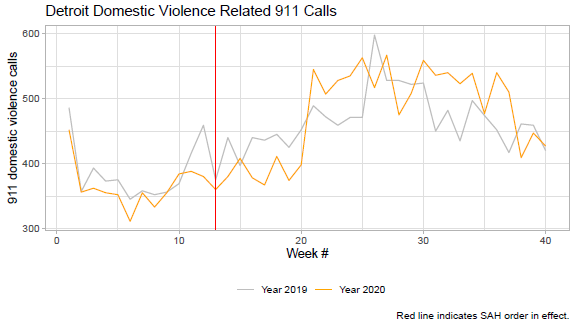
\includegraphics[width=0.9\textwidth,height=\textheight]{nm-ca_chart1.PNG}

\end{frame}

\begin{frame}{Sample visualizations from student projects (Liz Olson \&
Jenny Ostrowski)}
\protect\hypertarget{sample-visualizations-from-student-projects-liz-olson-jenny-ostrowski}{}

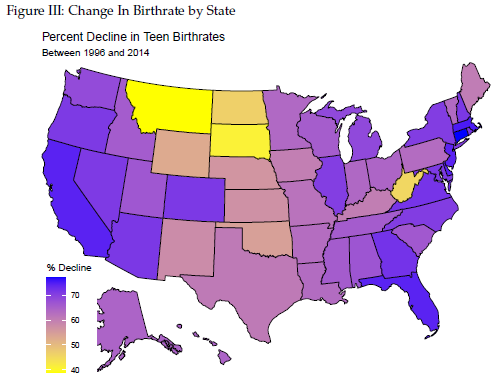
\includegraphics[width=0.9\textwidth,height=\textheight]{lo_jo_map1.PNG}

\end{frame}

\hypertarget{course-logistics}{%
\section{Course Logistics}\label{course-logistics}}

\begin{frame}{Syllabus and file management}
\protect\hypertarget{syllabus-and-file-management}{}

Course materials:

\begin{itemize}
\tightlist
\item
  All course files will be posted on the course website:
  \url{https://hreplots.github.io/U6614/}
\end{itemize}

\medskip

We'll be using Courseworks + Piazza for several purposes:

\begin{itemize}
\tightlist
\item
  hosting Zoom links for classes and recitation
\item
  weekly quizzes on asynchronous lessons
\item
  submitting assignments and project deliverables
\item
  course communications and discussion using Piazza (register
  \href{https://piazza.com/demo_login?nid=keiqq7y84rt5y2\&auth=6c81e06}{here})
\end{itemize}

\medskip

\end{frame}

\begin{frame}{Synchronous and asynchronous instruction}
\protect\hypertarget{synchronous-and-asynchronous-instruction}{}

\begin{enumerate}
\item
  Review asynchronous lessons in advance of class

  \begin{itemize}
  \tightlist
  \item
    will be posted to the course website by Thursday night
  \item
    class meetings will begin with a very short multiple choice quiz on
    the asynchronous material
  \end{itemize}
\end{enumerate}

\medskip

\begin{enumerate}
\setcounter{enumi}{1}
\item
  Synchronous instruction

  \begin{itemize}
  \tightlist
  \item
    short Zoom quiz
  \item
    discussion of data applications including assignments
  \item
    workshop-style instruction with R

    \begin{itemize}
    \tightlist
    \item
      prepare for class by downloading the week's R script \& data from
      the course website
    \item
      maintain a logical file structure to organize files
      (e.g.~Lectures/Lecture1)
    \end{itemize}
  \item
    we'll set \emph{community guidelines} for in-class participation/R
    support next week
  \end{itemize}
\end{enumerate}

\medskip

\textbf{Questions?}

\end{frame}

\hypertarget{rstudio}{%
\section{RStudio}\label{rstudio}}

\begin{frame}{What is RStudio?}
\protect\hypertarget{what-is-rstudio}{}

``\href{https://rstudio.com/products/rstudio/}{RStudio} is an integrated
development environment (IDE) for R. It includes a console,
syntax-highlighting editor that supports direct code execution, as well
as tools for plotting, history, debugging and workspace management.''

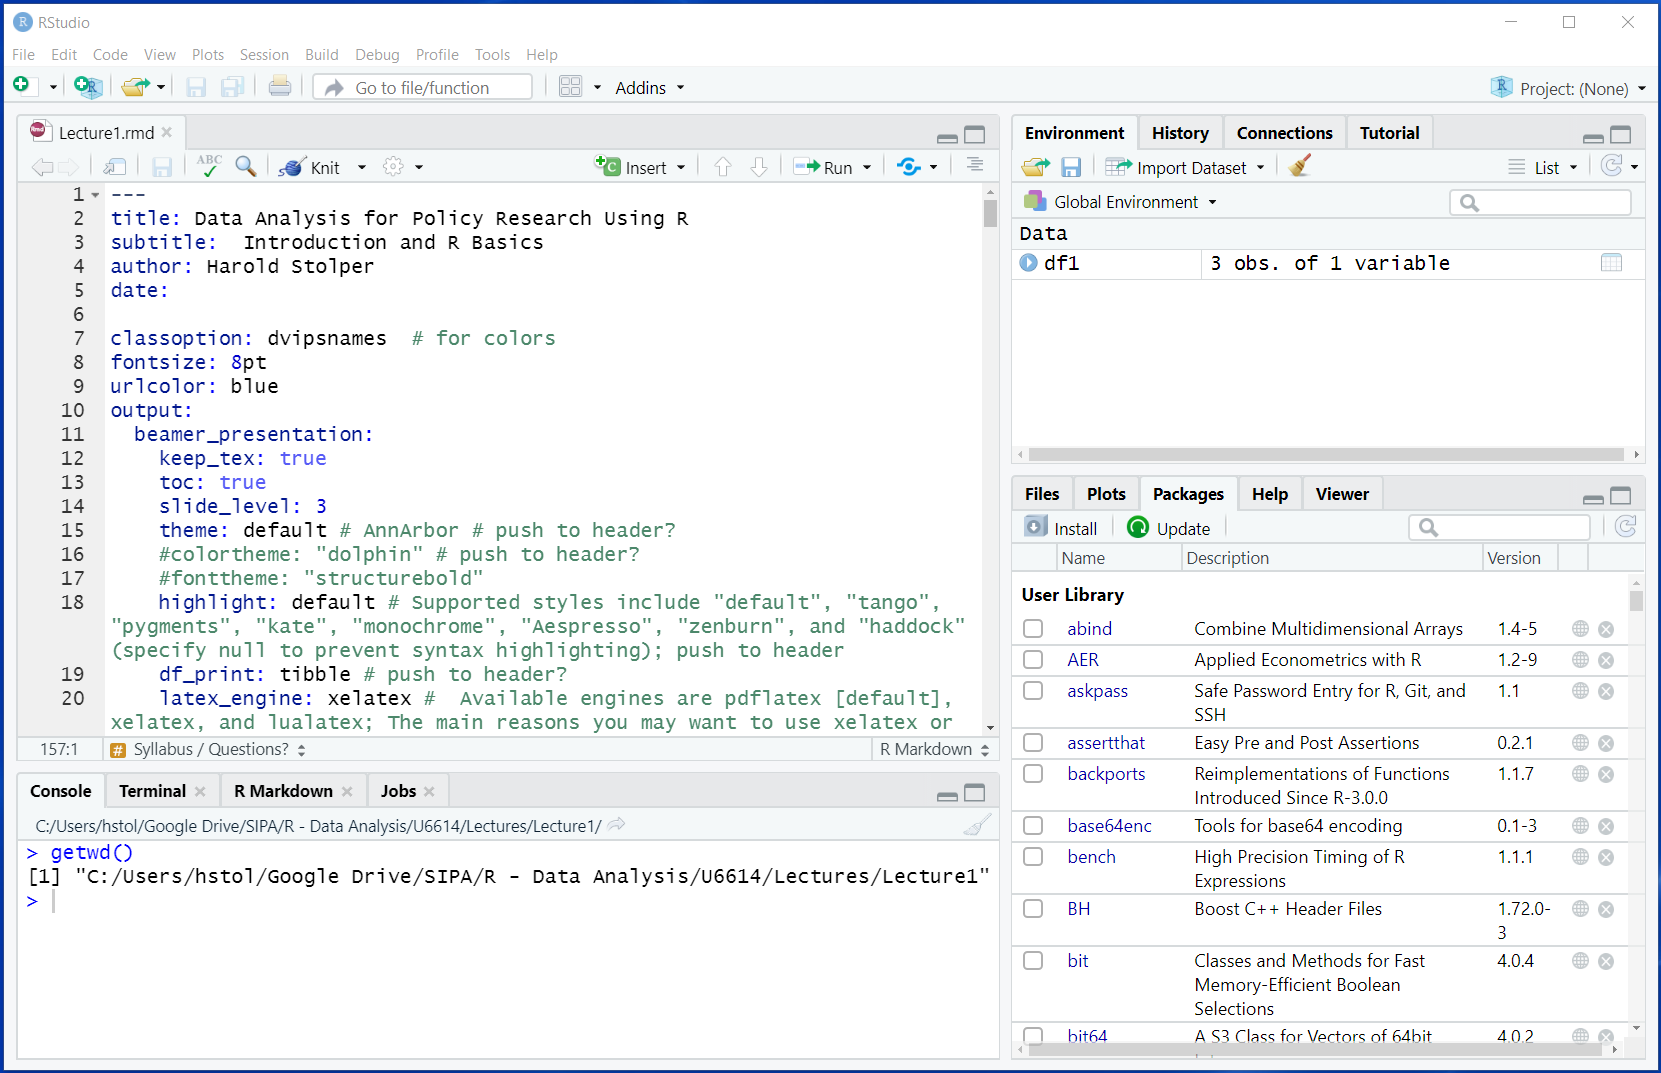
\includegraphics[width=0.9\textwidth,height=\textheight]{rstudio-capture1.PNG}

\end{frame}

\hypertarget{r-projects-and-directory-structure}{%
\section{R Projects and Directory
Structure}\label{r-projects-and-directory-structure}}

\begin{frame}[fragile]{Working directory}
\protect\hypertarget{working-directory}{}

R looks for files in your \textbf{working directory}

The function \texttt{getwd()} shows the current working directory (also
shown at the top of the RStudio console).

\begin{Shaded}
\begin{Highlighting}[]
\KeywordTok{getwd}\NormalTok{()}
\CommentTok{#> [1] "/Users/niyatimalhotra/Desktop/U6614/Lectures/Lecture1"}
\end{Highlighting}
\end{Shaded}

Function \texttt{list.files()} lists all files located in working
directory

\begin{Shaded}
\begin{Highlighting}[]
\KeywordTok{list.files}\NormalTok{()}
\end{Highlighting}
\end{Shaded}

\emph{Note that functions can accept arguments inside of parentheses,
but the simple functions shown above do not require any arguments.}

\end{frame}

\begin{frame}[fragile]{So what is the working directory?}
\protect\hypertarget{so-what-is-the-working-directory}{}

When you run code from the \textbf{R Console} or an \textbf{R Script},
or from \textbf{code chunks} in an R Markdown file (.rmd), the working
directory is\ldots{}

\begin{itemize}
\tightlist
\item
  the folder your file is saved in, or \ldots{}
\item
  if you are working within an \textbf{R Project}, the working directory
  is the main directory for the project (more on that shortly!)
\end{itemize}

\begin{Shaded}
\begin{Highlighting}[]
\KeywordTok{getwd}\NormalTok{()}
\CommentTok{#> [1] "/Users/niyatimalhotra/Desktop/U6614/Lectures/Lecture1"}
\end{Highlighting}
\end{Shaded}

\begin{itemize}
\tightlist
\item
  For this class we'll generally be using R projects to keep organized.
\end{itemize}

\end{frame}

\begin{frame}[fragile]{The path is how we refer to a directory}
\protect\hypertarget{the-path-is-how-we-refer-to-a-directory}{}

\textbf{Absolute file path}: a complete list of directories needed to
locate a file or folder.

\smallskip

\texttt{setwd("C:/Users/Harold\ Stolper/Google\ Drive/SIPA/R\ -\ Data\ Analysis/Fall\ 2020/Lectures/Lecture\ 1")}

\medskip

\textbf{Relative file path}: a way of indicating a given file location
relative to your working directory (note that they might be the same!)

\begin{itemize}
\tightlist
\item
  Assuming your current working directory is in the ``lecture2'' folder
  and you want to go up 2 levels to the ``Fall 2020'' folder, your
  relative file path would look something like this:
\end{itemize}

\texttt{setwd("../../")}

\medskip

\textbf{File path shortcuts:}

\begin{longtable}[]{@{}ll@{}}
\toprule
\textbf{Key} & \textbf{Description}\tabularnewline
\midrule
\endhead
\textasciitilde{} & tilde is a shortcut for the user's home
directory\tabularnewline
../ & moves up a level\tabularnewline
../../ & moves up two level\tabularnewline
\bottomrule
\end{longtable}

\end{frame}

\begin{frame}{What is an R project? Why are we using them?}
\protect\hypertarget{what-is-an-r-project-why-are-we-using-them}{}

What is an ``R project''?

\begin{itemize}
\tightlist
\item
  A file that keeps all ``project'' files organized together:

  \begin{itemize}
  \tightlist
  \item
    input data, R scripts, analytical results, and figures.
  \end{itemize}
\item
  When you open an R project, your working directory is automatically
  set to the directory where your R project lives.
\end{itemize}

Why will we be asking you to create and work with R projects?

\begin{itemize}
\tightlist
\item
  We want you to be able to run the R Markdown files (.rmd) used to
  generate each lecture.
\item
  Sometimes these .rmd files point to certain sub-folders
\item
  You can create or download an R project with directory structure
  (i.e.~organizing files and sub-folders in a particular way).
\item
  That way you'll be able to run .rmd files from your own computer that
  point to files in sub-folders without making any changes to
  file-paths.
\end{itemize}

\end{frame}

\hypertarget{r-basics}{%
\section{R Basics}\label{r-basics}}

\begin{frame}{Executing code in R}
\protect\hypertarget{executing-code-in-r}{}

Three ways to execute commands in R

\begin{enumerate}
\tightlist
\item
  \textbf{Console:} type/paste commands to run ``on the fly''
\item
  \textbf{R scripts} (.r files)

  \begin{itemize}
  \tightlist
  \item
    Just a text file full of R commands
  \item
    Can execute one command at a time, several commands at a time, or
    the entire script
  \end{itemize}
\item
  \textbf{Code chunks} in R Markdown (.rmd files)

  \begin{itemize}
  \tightlist
  \item
    Can execute one command at a time, one chunk at a time, or ``knit''
    the entire file into a document (html or pdf) that includes output
    from R code chunks
  \end{itemize}
\end{enumerate}

\end{frame}

\begin{frame}{Shortcuts for executing commands}
\protect\hypertarget{shortcuts-for-executing-commands}{}

\begin{enumerate}
\item
  Code chunks in R Markdown files

  \begin{itemize}
  \tightlist
  \item
    \textbf{Cmd/Ctrl + Enter}: execute highlighted line(s) within chunk
  \item
    \textbf{Cmd/Ctrl + Shift + k}: ``knit'' entire document
  \end{itemize}

  \medskip
\item
  R scripts (.r files)

  \begin{itemize}
  \tightlist
  \item
    \textbf{Cmd/Ctrl + Enter}: execute highlighted line(s)
  \item
    \textbf{Cmd/Ctrl + Shift + Enter} (without highlighting any lines):
    run entire script
  \end{itemize}
\end{enumerate}

\end{frame}

\begin{frame}[fragile]{Assignment in R}
\protect\hypertarget{assignment-in-r}{}

\textbf{Assignment} means assigning a value/set of values to an
``object''

\begin{itemize}
\tightlist
\item
  \texttt{\textless{}-} is the assignment operator

  \begin{itemize}
  \tightlist
  \item
    in other languages \texttt{=} is the assignment operator
  \end{itemize}
\item
  code is dense and hard to read, so it's good practice to put a space
  before and after assignment operator
\end{itemize}

\begin{Shaded}
\begin{Highlighting}[]
\CommentTok{# Create an object a and assign value}
\NormalTok{a <-}\StringTok{ }\DecValTok{5}
\NormalTok{a}
\CommentTok{#> [1] 5}

\CommentTok{# Create an object b and assign value}
\NormalTok{b <-}\StringTok{ "yay!"}
\NormalTok{b}
\CommentTok{#> [1] "yay!"}
\end{Highlighting}
\end{Shaded}

\emph{Note 1: comments start with one or more \texttt{\#} symbols}

\emph{Note 2: R is caps sensitive!}

\end{frame}

\begin{frame}{Objects and assignment}
\protect\hypertarget{objects-and-assignment}{}

R stores information in objects (like all ``object-oriented''
programming languages).

Some objects:

\begin{itemize}
\tightlist
\item
  numbers
\item
  character strings
\item
  vectors
\item
  matrices
\item
  lists
\item
  functions
\item
  plots
\item
  data frames (the datasets of R!)
\end{itemize}

Throughout this course, we'll be loading data objects to work with and
assigning values to new objects.

\end{frame}

\begin{frame}{Functions}
\protect\hypertarget{functions}{}

Functions do things to different objects. They often accept arguments --
we say we ``pass'' arguments to functions.

Functions are also objects themselves that can be ``called'' to do
things like:

\begin{itemize}
\tightlist
\item
  calculate and display statistics
\item
  generate output
\item
  display part or all of objects (e.g.~show some data)
\item
  manipulate objects (e.g.~create a new column of data)
\item
  extract information from objects (e.g.~the number of rows of data)
\end{itemize}

Base R includes lots of functions. We'll be working with base R
functions and handy functions from additional packages.

\end{frame}

\begin{frame}{Let's jump in!}
\protect\hypertarget{lets-jump-in}{}

Our goals for today's R workshop example are very modest:

\begin{itemize}
\tightlist
\item
  Create an R project including R script.
\item
  Look around and get our bearings.
\item
  Install and load a package
  (\href{https://www.gapminder.org/}{gapminder}).
\item
  Use base R functions to inspect a data frame included with this
  package.
\item
  Use some functions to perform some very basic analysis.
\item
  Assign results from our analysis to new objects and display them.
\end{itemize}

\end{frame}

\hypertarget{assignment-1}{%
\section{Assignment 1}\label{assignment-1}}

\begin{frame}{Assignment 1: submit an R script via CW before midnight
next Monday}
\protect\hypertarget{assignment-1-submit-an-r-script-via-cw-before-midnight-next-monday}{}

See \textbf{Assignment1.r} for details.

\medskip

Complete the assignment by including the necessary code, organized by
(sub)question, and use comments for non-code responses.

\medskip

Submit only your R script through CW using the following file name
syntax: \textbf{``Assignment1-YOURUNI.r''} via CW

\begin{itemize}
\tightlist
\item
  e.g.~``Assignment1-hbs2103.r''
\end{itemize}

\end{frame}

\begin{frame}{General assignment guidance}
\protect\hypertarget{general-assignment-guidance}{}

\begin{itemize}
\tightlist
\item
  \textbf{Use blank spaces liberally}, code is hard to read and spaces
  help!
\item
  \textbf{Use comments liberally} throughout your R script to describe
  your steps.
\item
  \textbf{Try to keep your code within the margins} to make it more
  readable.

  \begin{itemize}
  \tightlist
  \item
    R should know it can keep reading on the next line before
    executing\ldots{} unless you break after executable code
  \end{itemize}
\item
  Troubleshooting is a critical skill! Here are some tips and resources:

  \begin{itemize}
  \tightlist
  \item
    Consult the R script from today's class for examples.
  \item
    Get used to using R's built in documentation by using ``?''
  \item
    Use Google liberally to identify functions and find examples that
    work.
  \item
    When you're stuck, focus on finding examples to get your own code to
    work, even if you don't feel comfortable with all the syntax just
    yet.
  \end{itemize}
\item
  Consulting with others is fine! Copying, however, is not the way to
  learn to code or any language.

  \begin{itemize}
  \tightlist
  \item
    \textbf{Copied assignment submissions will result in a 0 for all
    parties.}
  \end{itemize}
\end{itemize}

\end{frame}

\hypertarget{course-expectations}{%
\section{Course expectations}\label{course-expectations}}

\begin{frame}{Course expectations}
\protect\hypertarget{course-expectations-1}{}

\begin{enumerate}
\item
  Review asynchronous (pre-class) lessons \textbf{before class}
\item
  Live attendance of class sessions is \textbf{required}

  \begin{itemize}
  \tightlist
  \item
    CW quizzes, in-class discussion and R workshop participation
  \end{itemize}
\item
  5 weekly assignments (``data memos'')
\item
  Data projects (starting week 5)

  \begin{itemize}
  \tightlist
  \item
    will culminate with a presentation and report at end of semester
  \item
    see syllabus for dates of intermediate deliverables
  \item
    3 required meetings with the teaching team to discuss progress
  \end{itemize}
\item
  Piazza discussion board participation
\item
  Recitation and office hours
\end{enumerate}

\medskip

\textbf{Questions?}

\end{frame}

\end{document}
